% =============================================================================
% Machine Learning-Based Rock Fragmentation Prediction from Blast Parameters
% Conference paper — IEEEtran conference class (works out of the box on
% Overleaf; if compiling locally without IEEEtran.cls installed, get it
% from CTAN: https://ctan.org/pkg/ieeetran)
% =============================================================================
\documentclass[conference]{IEEEtran}
\IEEEoverridecommandlockouts

\usepackage{amsmath,amssymb}
\usepackage{graphicx}
\usepackage{booktabs}
\usepackage{multirow}
\usepackage{siunitx}
\usepackage{url}
\usepackage{xcolor}
\usepackage{tcolorbox}
\usepackage{cite}

% ---------------------------------------------------------------------------
% PLACEHOLDER-RESULT NOTICE. Every number in Sections V-VIII is auto-
% generated by paper/make_tables.py from the CSV outputs of the Kaggle
% notebooks (notebooks/01..04). The tables shipped with this .tex file were
% produced by a FAST DEBUG run (N_TRIALS=3, 1 CV repeat) used only to check
% the pipeline end-to-end. DELETE THIS BOX (and re-run make_tables.py against
% the full Kaggle run, N_TRIALS=40 / n_repeats=10) before submission.
% ---------------------------------------------------------------------------
\newcommand{\PlaceholderNotice}{%
\begin{tcolorbox}[colback=red!5,colframe=red!60!black,title=DRAFT -- placeholder results,fontupper=\small]
The tables and figures below were generated by \texttt{paper/make\_tables.py}
from a \emph{fast debug} run of the Kaggle notebooks (3 Optuna trials, 1 CV
repeat) used only to verify the pipeline. \textbf{Re-run Notebooks 01--04 at
full settings on Kaggle, re-run \texttt{make\_tables.py}, and delete this box}
before the paper is submitted.
\end{tcolorbox}}

\begin{document}

\title{Machine Learning-Based Prediction of Rock Fragmentation from Blast
Design Parameters: A Leakage-Aware Benchmark on a Multi-Mine Database}

\author{
\IEEEauthorblockN{Author Name\IEEEauthorrefmark{1}, Co-Author Name\IEEEauthorrefmark{1}}
\IEEEauthorblockA{\IEEEauthorrefmark{1}Department of Mining Engineering, University/Institute Name, City, Country\\
Email: author@example.edu}
}

\maketitle

\begin{abstract}
Accurate prediction of the mean fragment size ($X_{50}$) resulting from
bench blasting is central to mine-to-mill optimisation, since fragmentation
governs downstream loading, hauling, crushing and grinding costs. Empirical
models such as the Kuznetsov and Kuz--Ram equations are widely used but do
not capture the strongly non-linear relationship between blast-design
ratios, explosive loading and rock-mass properties. This paper presents a
leakage-aware machine-learning benchmark for $X_{50}$ prediction using a
database of 110 real bench blasts from ten mines and quarries in five
countries (Spain, Turkey, Indonesia, India and the USA), compiled from the
published work of Hudaverdi, Kulatilake and Kuzu. Seven blast-design,
explosive and rock-property ratios (S/B, H/B, B/D, T/B, powder factor,
in-situ block size and elastic modulus) are used to predict $X_{50}$ with
Random Forest, Extra Trees, XGBoost, LightGBM, CatBoost, Support Vector
Regression, Gaussian Process Regression and an Artificial Neural Network,
benchmarked against the Kuznetsov equation and a multivariate power-law
regression. Unlike prior studies on this database, which report a single
$\sim$12-blast test split, we evaluate every model under three protocols:
the original paper split, repeated duplicate-aware grouped $k$-fold
cross-validation, and leave-one-site-out cross-validation, with nested
hyper-parameter tuning and a corrected resampled $t$-test for statistical
significance. We further quantify feature importance with SHAP and
permutation methods, check the physical consistency of the learned
trends, and provide split-conformal prediction intervals. Results show
[\emph{RESULT: fill in from Table~\ref{tab:t4_results_p2} after the full
Kaggle run}], and reveal that model performance degrades substantially
when generalising to an unseen mine, exposing a site-identity confound
(elastic modulus and burden-to-diameter ratio are nearly constant within a
site) that is masked by the evaluation protocols used in prior work.
\end{abstract}

\begin{IEEEkeywords}
rock fragmentation, blast design, machine learning, random forest, XGBoost,
support vector regression, artificial neural network, Kuz--Ram model, SHAP
\end{IEEEkeywords}

% =============================================================================
\section{Introduction}
% =============================================================================
Rock fragmentation is the size distribution of broken rock produced by a
blast. It is the single blasting outcome with the largest downstream
economic impact: coarse fragmentation increases secondary breakage, reduces
loader and excavator productivity, and lowers crusher and mill throughput,
whereas excessively fine fragmentation wastes explosive energy
\cite{kulatilake2010}. The ``mine-to-mill'' philosophy explicitly optimises
blast design to minimise the combined cost of drilling, blasting, loading
and comminution rather than blasting cost alone.

The most widely used engineering tool for fragmentation prediction is the
Kuznetsov equation \cite{kuznetsov1973}, later developed into the Kuz--Ram
model by Cunningham \cite{cunningham1983,cunningham2005}, which combines an
empirical mean-fragment-size relation with the Rosin--Rammler size
distribution and a uniformity index. While easy to parameterise, Kuz--Ram
relies on a coarse, subjectively assigned rock factor $A$, does not use
measured rock-mass stiffness, and is known to under-predict the fines
fraction \cite{gebretsadik2024}. Because the true relationship between
blast-design parameters and fragmentation is highly non-linear and involves
a heterogeneous, anisotropic rock mass, several authors have applied
machine learning (ML) to this problem, most influentially the multivariate
regression (MVR) and back-propagation artificial neural network (ANN) study
of Kulatilake et al.\ \cite{kulatilake2010} and the underlying blast
database compiled by Hudaverdi et al.\ \cite{hudaverdi2011}. Subsequent
studies re-used this database with support vector regression (SVR)
\cite{shi2012} and a hybrid multilayer ANN/SVR architecture
\cite{amoako2022}, and newer studies applied Random Forest, XGBoost and
deep ANNs to a separate 219-blast limestone-quarry dataset
\cite{gebretsadik2024}.

\subsection{Gaps in the existing literature}
Reviewing this body of work reveals three recurring limitations, all of
which we address in this paper:
\begin{enumerate}
  \item \textbf{Evaluation instability.} Every study on the Hudaverdi
  database reports results on a single held-out split of only 12--13
  blasts \cite{kulatilake2010,shi2012,amoako2022}. With so few test points,
  the reported $R^2$ has very high variance and is not directly comparable
  across papers.
  \item \textbf{Duplicate and near-duplicate leakage.} Several blasts in
  the database share \emph{identical} input ratios (e.g.\ blasts En3/En5,
  En8/En9) but different measured $X_{50}$, reflecting natural field
  variability; if such duplicates are split across train and test folds by
  an ordinary random $k$-fold, a memorising model can appear to generalise
  when it is in fact recalling a near-identical training row.
  \item \textbf{Site confounding.} Rock elastic modulus $E$ and the
  burden-to-hole-diameter ratio $B/D$ are almost constant within a given
  mine (Section~\ref{sec:data}), so a model can partly ``recognise the
  mine'' rather than learn blast physics; none of the prior studies test
  generalisation to a mine absent from training.
\end{enumerate}

\subsection{Contributions}
This paper makes the following contributions:
\begin{itemize}
  \item We assemble and publicly release the largest available version of
  this database (110 real, field-measured blasts, ten sites, five
  countries; no synthetic or simulated data), cross-checked against the
  originally published tables with two corrected values (Section
  \ref{sec:data}).
  \item We introduce a \textbf{duplicate-aware, grouped, repeated}
  cross-validation protocol and a \textbf{leave-one-site-out} protocol
  alongside the conventional paper-split protocol, and report a
  \textbf{statistical significance test} (corrected resampled $t$-test
  \cite{nadeau2003}) between models -- absent from all prior work on this
  problem.
  \item We benchmark eight ML regressors against the Kuznetsov equation and
  MVR with nested nested hyper-parameter tuning, and quantify feature
  importance with SHAP \cite{lundberg2017}, permutation importance and
  partial dependence, checking learned trends against blasting-physics
  expectations.
  \item We provide split-conformal prediction intervals and a simple
  powder-factor design tool, and release fully reproducible Kaggle
  notebooks and a table-generation script so every number in this paper is
  traceable to a specific, versioned notebook run.
\end{itemize}

% =============================================================================
\section{Related Work}
% =============================================================================
Table~\ref{tab:related} summarises the studies most closely related to this
work; all use variants of the same underlying blast database.

\begin{table}[t]
\caption{Summary of closely related studies}
\label{tab:related}
\centering
\small
\begin{tabular}{p{1.5cm}p{1.6cm}p{1.9cm}p{1.9cm}}
\toprule
\textbf{Study} & \textbf{Data} & \textbf{Models} & \textbf{Reported test result} \\
\midrule
Hudaverdi et al.\ 2011 \cite{hudaverdi2011} & 97+13 & MVR (2 groups) & $R^2\!\approx\!0.82$ (13-blast valid.) \\
Kulatilake et al.\ 2010 \cite{kulatilake2010} & 90+12 & BP-ANN, MVR, Kuznetsov & ANN $R^2{=}0.94$, MVR $0.82$, Kuznetsov $0.57$ \\
Shi et al.\ 2012 \cite{shi2012} & 90/12 & SVR & ``acceptable accuracy'' \\
Amoako et al.\ 2022 \cite{amoako2022} & 90/12 & deep ANN, SVR & ANN $r^2{=}0.87$, SVR $r^2{=}0.81$, Kuznetsov $0.58$ \\
Gebretsadik et al.\ 2024 \cite{gebretsadik2024} & 219 (1 quarry, private) & RF, SVR, XGB, ANN & RF $R^2{=}0.94$ (test) \\
\bottomrule
\end{tabular}
\end{table}

All five studies fit models on the same $\sim$90--105 development blasts
and test on a disjoint set of only 12--13 blasts drawn from the same mines;
none report cross-validated variance, a statistical comparison between
models, or generalisation to an unseen site. Gebretsadik et al.\
\cite{gebretsadik2024} use a larger, single-quarry dataset with different
input features (drill diameter, number of holes, specific drilling) and a
different target definition (percentage fragmentation rather than
$X_{50}$ in metres); because their raw data are not public, we treat their
reported results as a literature reference point only, not as additional
training data.

% =============================================================================
\section{Database}
\label{sec:data}
% =============================================================================
\subsection{Provenance}
The database used in this study is drawn from real, measured bench blasts
compiled and published by Hudaverdi, Kulatilake and Kuzu
\cite{hudaverdi2011} and subsequently used for neural-network modelling by
Kulatilake et al.\ \cite{kulatilake2010}. \textbf{No synthetic, simulated
or augmented data are used at any stage of training or testing.} The
database combines blasts reported in the literature
\cite{kulatilake2010,hudaverdi2011} with a machine-readable transcription
maintained on GitHub \cite{blastdesigngithub}, which we cross-checked value
by value against the 90 blasts published directly in
\cite{kulatilake2010}: two discrepancies were found and corrected against
the published tables (blast Oz7 powder factor $0.53\!\to\!0.70$~kg/m$^3$;
blast Ad22 elastic modulus $15.0\!\to\!16.9$~GPa). The resulting
110-blast, 10-site database is released alongside this paper together with
a full provenance log (\texttt{data/DATA\_NOTES.txt}).

\begin{table}[t]
\centering
\caption{Mines and quarries represented in the database}
\label{tab:sites}
\begin{tabular}{lllllr}
\toprule
site & mine & country & rock\_type & E\_group & n\_blasts \\
\midrule
Akdaglar & Akdaglar Quarry & Turkey (Istanbul) & Sandstone (aggregate) & G2\_low\_E & 25 \\
Enusa & Enusa Mine & Spain & Uranium ore (schistose, folded) & G1\_high\_E & 13 \\
Mrica & Mrica Quarry & Indonesia & Andesite & G2\_low\_E & 12 \\
Dongri-Buzurg & Dongri-Buzurg Mine & India & Manganese ore (micaceous/muscovite schist) & G2\_low\_E & 10 \\
Reocin & Reocin Mine & Spain & Zinc ore & G1\_high\_E & 10 \\
Murgul & Murgul Copper Mine & Turkey & Dacite / altered dacite (copper) & G1\_high\_E & 9 \\
Ozmert & Ozmert Quarry & Turkey (Istanbul) & Sandstone (aggregate) & G2\_low\_E & 9 \\
Soma & Soma Basin Coal Mine & Turkey & Coal & G2\_low\_E & 8 \\
Miami & Miami Mine & USA (Arizona) & Pinal schist & G2\_low\_E & 7 \\
Reocin-UG & Reocin Mine (Underground) & Spain & Zinc ore & G1\_high\_E & 7 \\
\bottomrule
\end{tabular}

\end{table}

\subsection{Features and target}
Seven dimensionless ratios and physical quantities, identical to those used
by \cite{hudaverdi2011,kulatilake2010,shi2012,amoako2022}, are used as
inputs: spacing-to-burden ratio $S/B$, bench-height-to-burden ratio $H/B$,
burden-to-hole-diameter ratio $B/D$, stemming-to-burden ratio $T/B$, powder
factor $P_f$ (kg/m$^3$), in-situ block size $X_B$ (m), and rock elastic
modulus $E$ (GPa). The target is the measured mean fragment size
$X_{50}$ (m), obtained in the source studies by digital image analysis of
the muck pile. Table~\ref{tab:descriptive} gives descriptive statistics.

\begin{table}[t]
\centering
\caption{Descriptive statistics of the input and target variables (110 blasts)}
\label{tab:descriptive}
\begin{tabular}{lrrrrrrrrr}
\toprule
 & count & mean & std & min & 25\% & 50\% & 75\% & max & skew \\
Variable &  &  &  &  &  &  &  &  &  \\
\midrule
S\_B & 110.000 & 1.185 & 0.114 & 1.000 & 1.130 & 1.200 & 1.248 & 1.750 & 1.003 \\
H\_B & 110.000 & 3.338 & 1.602 & 1.330 & 2.070 & 2.815 & 4.688 & 6.820 & 0.517 \\
B\_D & 110.000 & 27.415 & 4.943 & 17.980 & 24.720 & 27.270 & 30.300 & 39.470 & 0.066 \\
T\_B & 110.000 & 1.258 & 0.672 & 0.500 & 0.830 & 1.110 & 1.400 & 4.670 & 2.623 \\
Pf & 110.000 & 0.541 & 0.239 & 0.220 & 0.352 & 0.480 & 0.690 & 1.260 & 1.354 \\
XB & 110.000 & 1.092 & 0.530 & 0.020 & 0.692 & 1.030 & 1.522 & 2.350 & 0.092 \\
E & 110.000 & 29.165 & 17.824 & 9.570 & 15.000 & 16.900 & 45.000 & 60.000 & 0.498 \\
X50 & 110.000 & 0.299 & 0.184 & 0.020 & 0.170 & 0.230 & 0.395 & 0.960 & 1.213 \\
\bottomrule
\end{tabular}

\end{table}

\subsection{Data quality considerations}
\label{sec:leakage}
Two properties of the database directly motivate our evaluation design
(Section~\ref{sec:methods}):
\begin{itemize}
  \item \textbf{Duplicate inputs.} Several blasts share identical values of
  all seven inputs but differ in measured $X_{50}$ (e.g.\ En3 vs.\ En5,
  Mg5 vs.\ Mg7), reflecting genuine field-measurement variability. The
  pooled within-cluster standard deviation of $X_{50}$ is an
  \emph{irreducible noise floor} that no model can beat on average, and we
  quote it alongside benchmark RMSE.
  \item \textbf{Site clustering.} $E$ is constant within each mine by
  construction (it represents the site's rock stiffness) and $B/D$ varies
  little within a site because hole diameter and burden are standard
  operating parameters at a given quarry. Figure~\ref{fig:scatter}
  illustrates this clustering.
\end{itemize}

\begin{figure}[t]
\centering
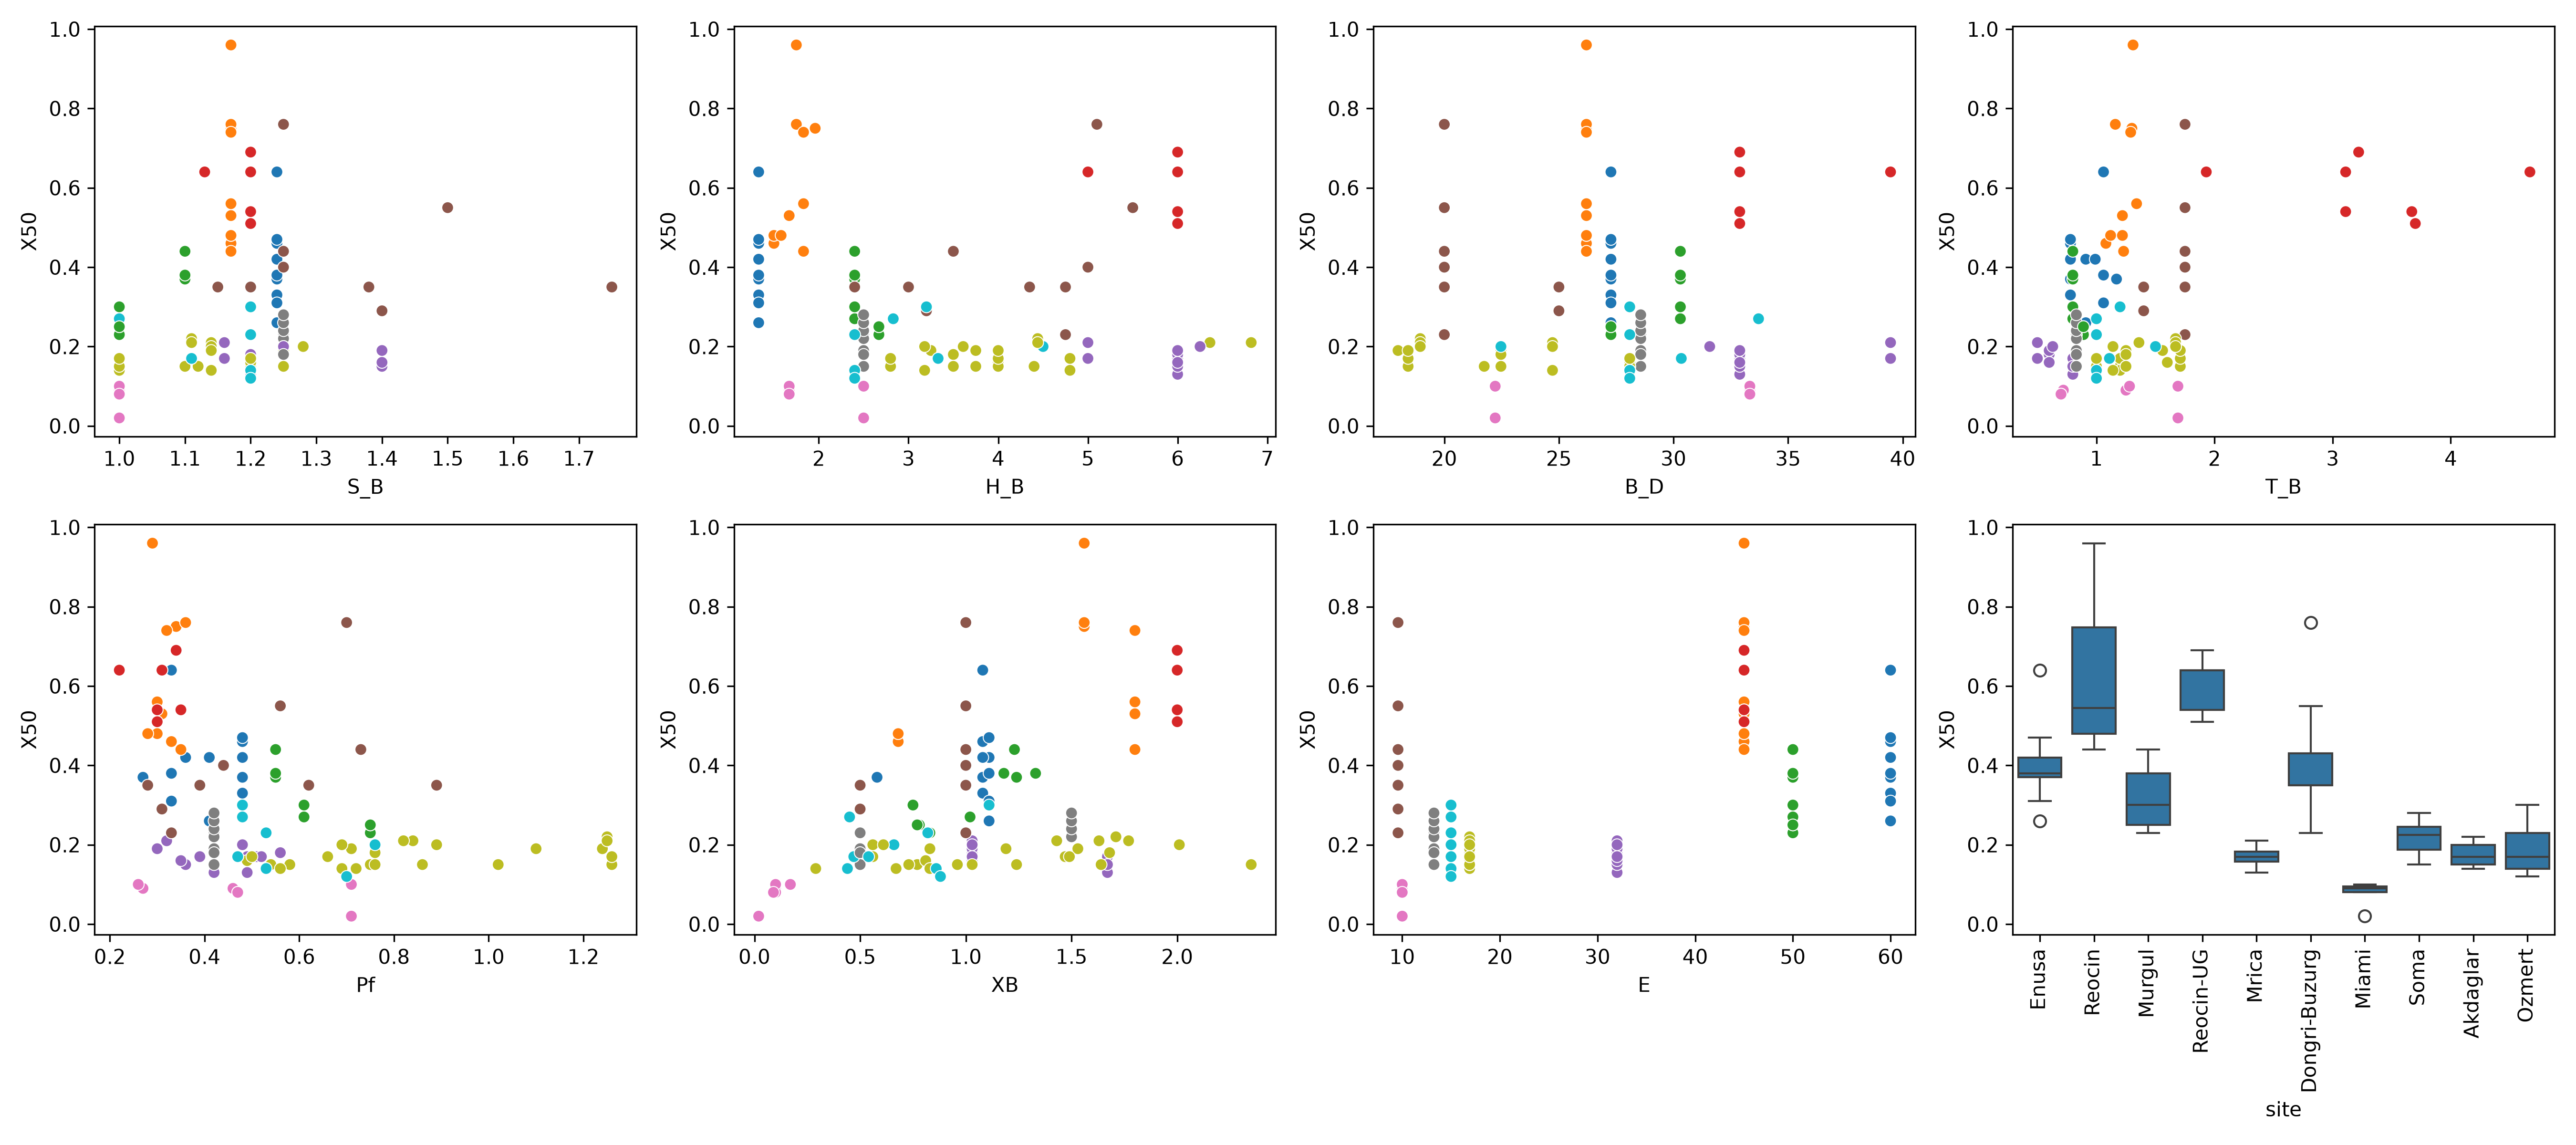
\includegraphics[width=\columnwidth]{figures/F4_scatter_by_site.png}
\caption{$X_{50}$ versus each blast-design input, coloured by mine site.
Several inputs (notably $E$ and $B/D$) show strong within-site clustering.}
\label{fig:scatter}
\end{figure}

\begin{figure}[t]
\centering
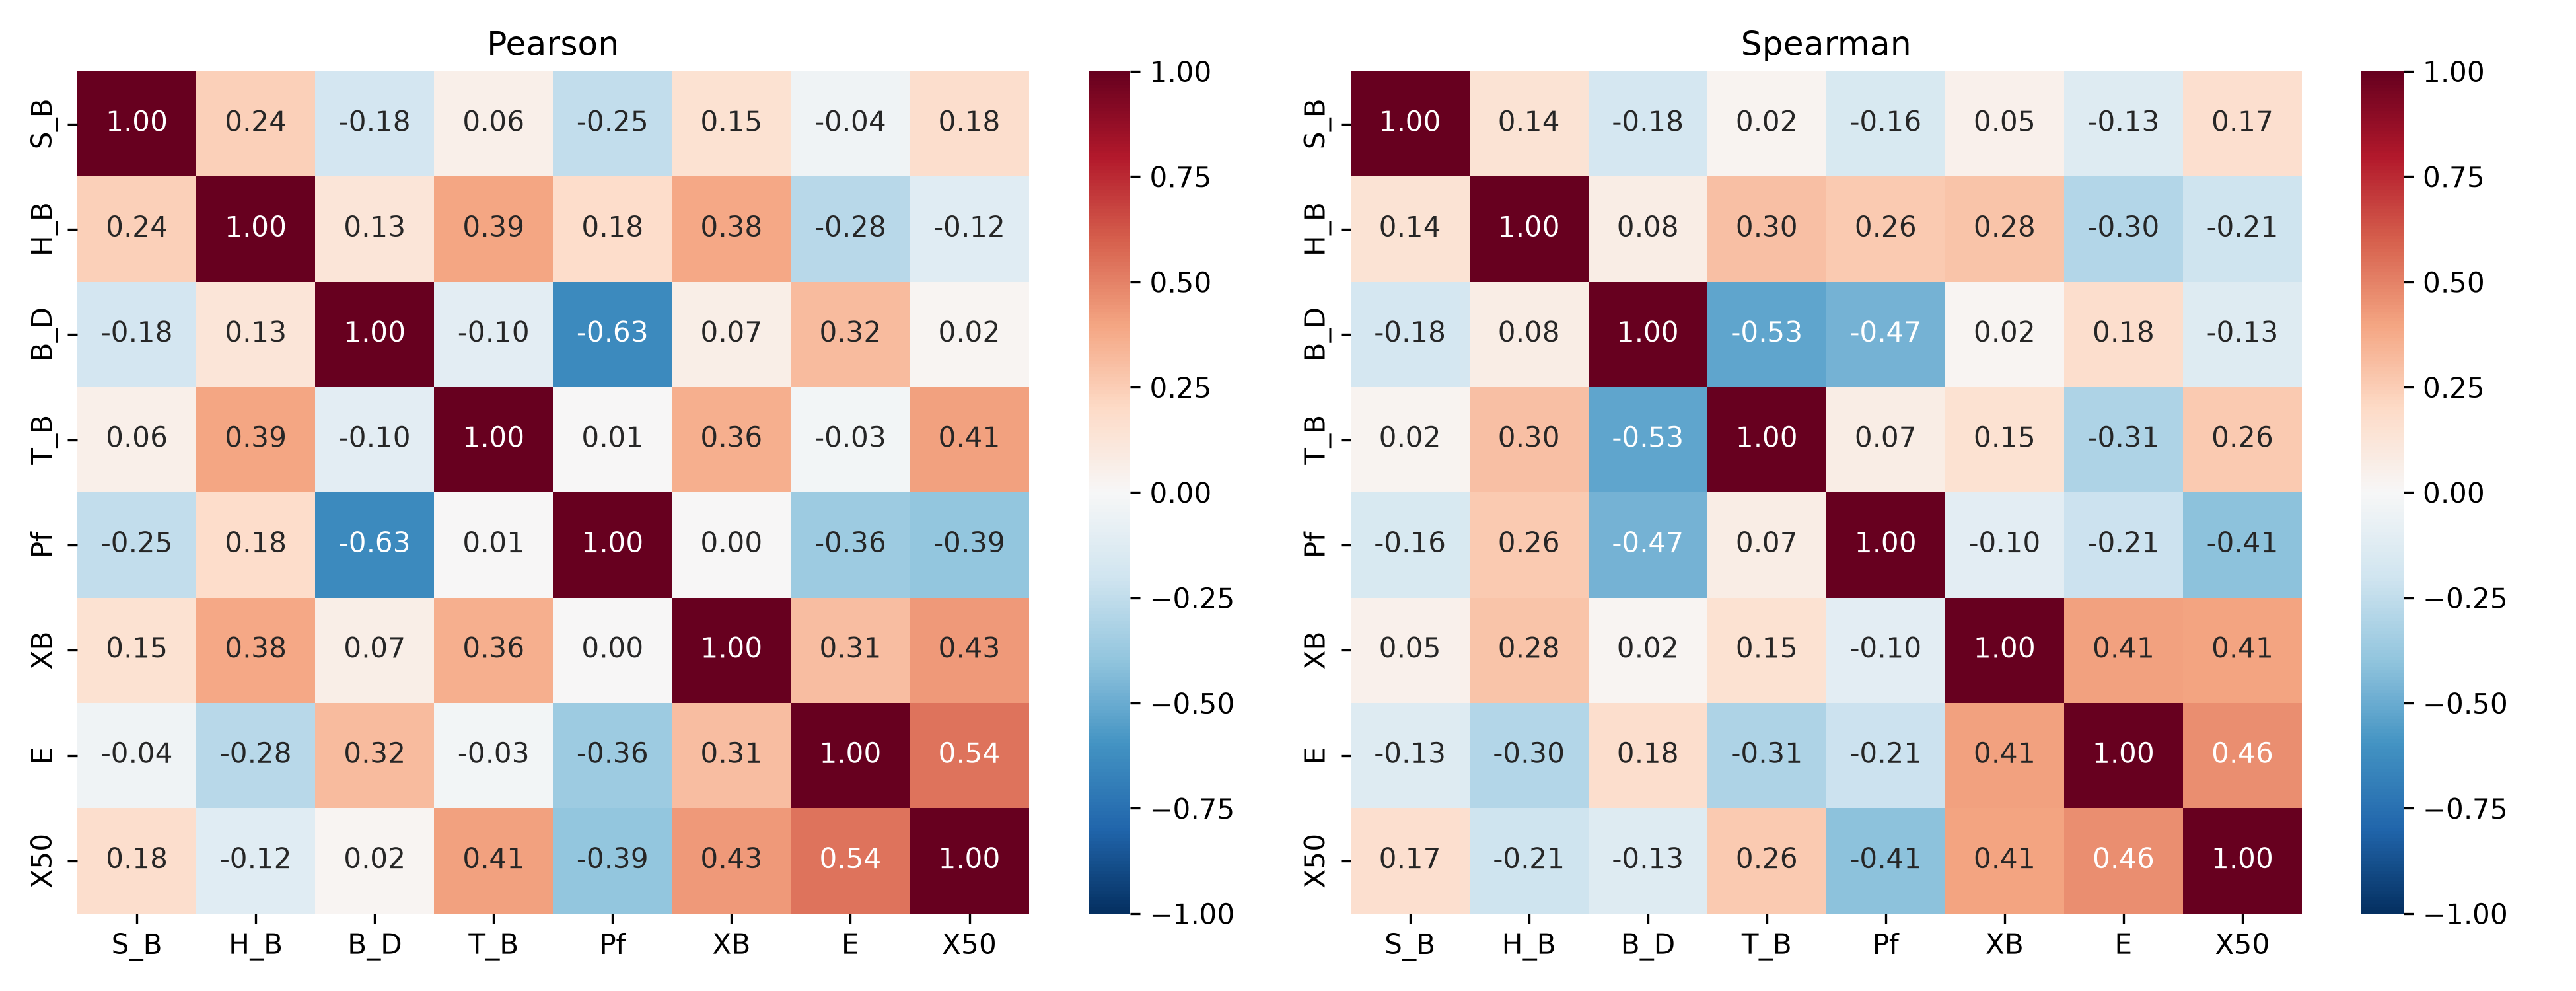
\includegraphics[width=\columnwidth]{figures/F3_correlation.png}
\caption{Pearson and Spearman correlation of the seven inputs with $X_{50}$.}
\label{fig:corr}
\end{figure}

% =============================================================================
\section{Methodology}
\label{sec:methods}
% =============================================================================
\subsection{Evaluation protocols}
All models are evaluated under three protocols:

\textbf{P1 -- paper split.} 97 development blasts / 13 original validation
blasts, reproducing the split used in \cite{hudaverdi2011,kulatilake2010},
enabling direct comparison with published numbers.

\textbf{P2 -- repeated grouped $k$-fold CV (main protocol).} Ten repeats of
5-fold cross-validation over all 110 blasts. Blasts sharing identical
inputs (Section~\ref{sec:leakage}) are assigned to a common group id and
\texttt{GroupKFold} guarantees they are never split across train/test,
eliminating duplicate-row leakage.

\textbf{P3 -- leave-one-site-out (LOSO).} Each of the ten mines is held out
in turn; this is the realistic deployment scenario of predicting
fragmentation at a site with no training history, and is, to our
knowledge, not evaluated in any prior study on this database.

Hyper-parameters are tuned with Optuna (Tree-structured Parzen Estimator,
40 trials) on an \emph{inner} 5-fold grouped cross-validation of the
training fold only, so the outer test fold is never used for model
selection. Reported metrics are $R^2$, RMSE, MAE, MAPE, variance accounted
for (VAF) and the $a_{20}$-index (fraction of predictions within $\pm20\%$
of the measured value).

\subsection{Baselines}
\textbf{Kuznetsov / Kuz--Ram.} This model requires absolute burden,
spacing, bench height and per-hole charge mass, which are not present in
the ratio-based database; we therefore compare against the Kuznetsov
predictions already published in \cite{kulatilake2010} for the 12 shared
validation blasts (Section~\ref{sec:results}), consistent with the
practice in \cite{amoako2022}.

\textbf{Multivariate regression (MVR).} Following
\cite{hudaverdi2011,kulatilake2010}, we fit the power-law form
$\ln X_{50} = \ln a + \sum_i b_i \ln x_i$ by ordinary least squares.

\subsection{Machine-learning models}
Random Forest \cite{breiman2001}, Extra Trees, XGBoost
\cite{chen2016xgboost}, LightGBM, CatBoost, Support Vector Regression
\cite{cortes1995svr} (RBF kernel), Gaussian Process Regression, and a
multilayer perceptron ANN (1--3 hidden layers, L-BFGS solver) are compared,
each optionally fit on $\log X_{50}$ via a target transform. A Ridge
regression and a mean predictor serve as lower-bound sanity checks.

\subsection{Statistical testing}
For the P2 protocol, we compare the best model (lowest mean RMSE) against
every other model using the corrected resampled $t$-test of Nadeau \&
Bengio \cite{nadeau2003}, which accounts for the correlation between
overlapping cross-validation folds, with Holm correction for multiple
comparisons, and a Friedman omnibus test across all models.

\subsection{Interpretability and uncertainty}
Feature importance is quantified with SHAP TreeExplainer (tree models) and
KernelExplainer (SVR, ANN) \cite{lundberg2017}, permutation importance, and
partial dependence / ICE plots. We check whether the sign of each learned
trend agrees with blasting-physics expectations (higher powder factor
$\rightarrow$ finer $X_{50}$; higher stemming ratio and larger in-situ
block size $\rightarrow$ coarser $X_{50}$). Split-conformal prediction
intervals (90\%) are computed from out-of-fold residuals, with empirical
coverage reported under P2 and P3.

% =============================================================================
\section{Results}
\label{sec:results}
% =============================================================================
\PlaceholderNotice

\subsection{Main benchmark}
Table~\ref{tab:t4_results_p1} reports results under the paper-split
protocol P1; Table~\ref{tab:t4_results_p2} under the main repeated grouped
CV protocol P2; Table~\ref{tab:t4_results_p3_pooled} under leave-one-site-out.

\begin{table}[t]
\centering
\caption{Results under the paper-split protocol (P1)}
\label{tab:t4_results_p1}
\small
\begin{tabular}{lllllll}
\toprule
 & R2 & RMSE & MAE & MAPE & VAF & a20 \\
Model &  &  &  &  &  &  \\
\midrule
LGBM & NaN & NaN & NaN & NaN & NaN & NaN \\
RF & NaN & NaN & NaN & NaN & NaN & NaN \\
CatB & NaN & NaN & NaN & NaN & NaN & NaN \\
XGB & NaN & NaN & NaN & NaN & NaN & NaN \\
ET & NaN & NaN & NaN & NaN & NaN & NaN \\
Ridge & NaN & NaN & NaN & NaN & NaN & NaN \\
GPR & NaN & NaN & NaN & NaN & NaN & NaN \\
ANN & NaN & NaN & NaN & NaN & NaN & NaN \\
MVR & NaN & NaN & NaN & NaN & NaN & NaN \\
SVR & NaN & NaN & NaN & NaN & NaN & NaN \\
Mean & NaN & NaN & NaN & NaN & NaN & NaN \\
\bottomrule
\end{tabular}

\end{table}

\begin{table}[t]
\centering
\caption{Results under repeated grouped 5-fold CV (P2, main protocol)}
\label{tab:t4_results_p2}
\small
\begin{tabular}{lllllll}
\toprule
 & R2 & RMSE & MAE & MAPE & VAF & a20 \\
Model &  &  &  &  &  &  \\
\midrule
CatB & 0.725 $\pm$ 0.145 & 0.084 $\pm$ 0.036 & 0.058 $\pm$ 0.016 & 25.029 $\pm$ 11.413 & 75.785 $\pm$ 12.333 & 0.609 $\pm$ 0.059 \\
RF & 0.7 $\pm$ 0.186 & 0.085 $\pm$ 0.035 & 0.06 $\pm$ 0.018 & 25.271 $\pm$ 13.524 & 72.506 $\pm$ 18.684 & 0.594 $\pm$ 0.069 \\
XGB & 0.658 $\pm$ 0.172 & 0.093 $\pm$ 0.034 & 0.063 $\pm$ 0.019 & 24.949 $\pm$ 8.315 & 68.671 $\pm$ 16.55 & 0.609 $\pm$ 0.044 \\
GPR & 0.515 $\pm$ 0.56 & 0.094 $\pm$ 0.023 & 0.063 $\pm$ 0.012 & 23.919 $\pm$ 6.233 & 56.02 $\pm$ 52.373 & 0.638 $\pm$ 0.053 \\
ET & 0.672 $\pm$ 0.19 & 0.094 $\pm$ 0.049 & 0.061 $\pm$ 0.026 & 22.323 $\pm$ 10.32 & 70.679 $\pm$ 16.57 & 0.63 $\pm$ 0.13 \\
LGBM & 0.62 $\pm$ 0.245 & 0.095 $\pm$ 0.03 & 0.065 $\pm$ 0.013 & 27.784 $\pm$ 10.143 & 67.0 $\pm$ 21.163 & 0.62 $\pm$ 0.061 \\
MVR & 0.506 $\pm$ 0.241 & 0.113 $\pm$ 0.045 & 0.084 $\pm$ 0.026 & 30.259 $\pm$ 6.753 & 55.454 $\pm$ 21.628 & 0.391 $\pm$ 0.074 \\
Ridge & 0.441 $\pm$ 0.414 & 0.113 $\pm$ 0.046 & 0.083 $\pm$ 0.028 & 38.53 $\pm$ 16.578 & 54.571 $\pm$ 25.317 & 0.447 $\pm$ 0.102 \\
SVR & 0.441 $\pm$ 0.233 & 0.121 $\pm$ 0.04 & 0.083 $\pm$ 0.022 & 30.869 $\pm$ 10.457 & 47.466 $\pm$ 23.216 & 0.481 $\pm$ 0.019 \\
ANN & -0.088 $\pm$ 1.057 & 0.157 $\pm$ 0.114 & 0.092 $\pm$ 0.044 & 38.979 $\pm$ 22.318 & -6.883 $\pm$ 103.358 & 0.533 $\pm$ 0.112 \\
Mean & -0.39 $\pm$ 0.778 & 0.184 $\pm$ 0.039 & 0.151 $\pm$ 0.022 & 74.926 $\pm$ 24.49 & -0.0 $\pm$ 0.0 & 0.138 $\pm$ 0.089 \\
\bottomrule
\end{tabular}

\end{table}

\begin{table}[t]
\centering
\caption{Results under leave-one-site-out CV (P3, pooled out-of-fold)}
\label{tab:t4_results_p3_pooled}
\small
\begin{tabular}{lrrrrrr}
\toprule
 & R2 & RMSE & MAE & MAPE & VAF & a20 \\
Model &  &  &  &  &  &  \\
\midrule
Ridge & 0.131 & 0.171 & 0.130 & 59.933 & 17.952 & 0.264 \\
ET & 0.106 & 0.174 & 0.139 & 72.945 & 11.914 & 0.200 \\
MVR & 0.099 & 0.174 & 0.136 & 62.470 & 10.852 & 0.264 \\
LGBM & 0.042 & 0.180 & 0.135 & 71.520 & 4.436 & 0.273 \\
CatB & -0.016 & 0.185 & 0.146 & 74.147 & -0.990 & 0.209 \\
RF & -0.026 & 0.186 & 0.138 & 75.800 & 1.987 & 0.282 \\
XGB & -0.141 & 0.196 & 0.152 & 75.950 & -14.111 & 0.236 \\
SVR & -0.155 & 0.197 & 0.144 & 61.395 & -15.316 & 0.246 \\
Mean & -0.204 & 0.202 & 0.167 & 84.097 & -20.359 & 0.154 \\
GPR & -0.421 & 0.219 & 0.174 & 75.759 & -41.222 & 0.154 \\
ANN & -1.558 & 0.294 & 0.222 & 88.845 & -155.699 & 0.164 \\
\bottomrule
\end{tabular}

\end{table}

\begin{figure}[t]
\centering
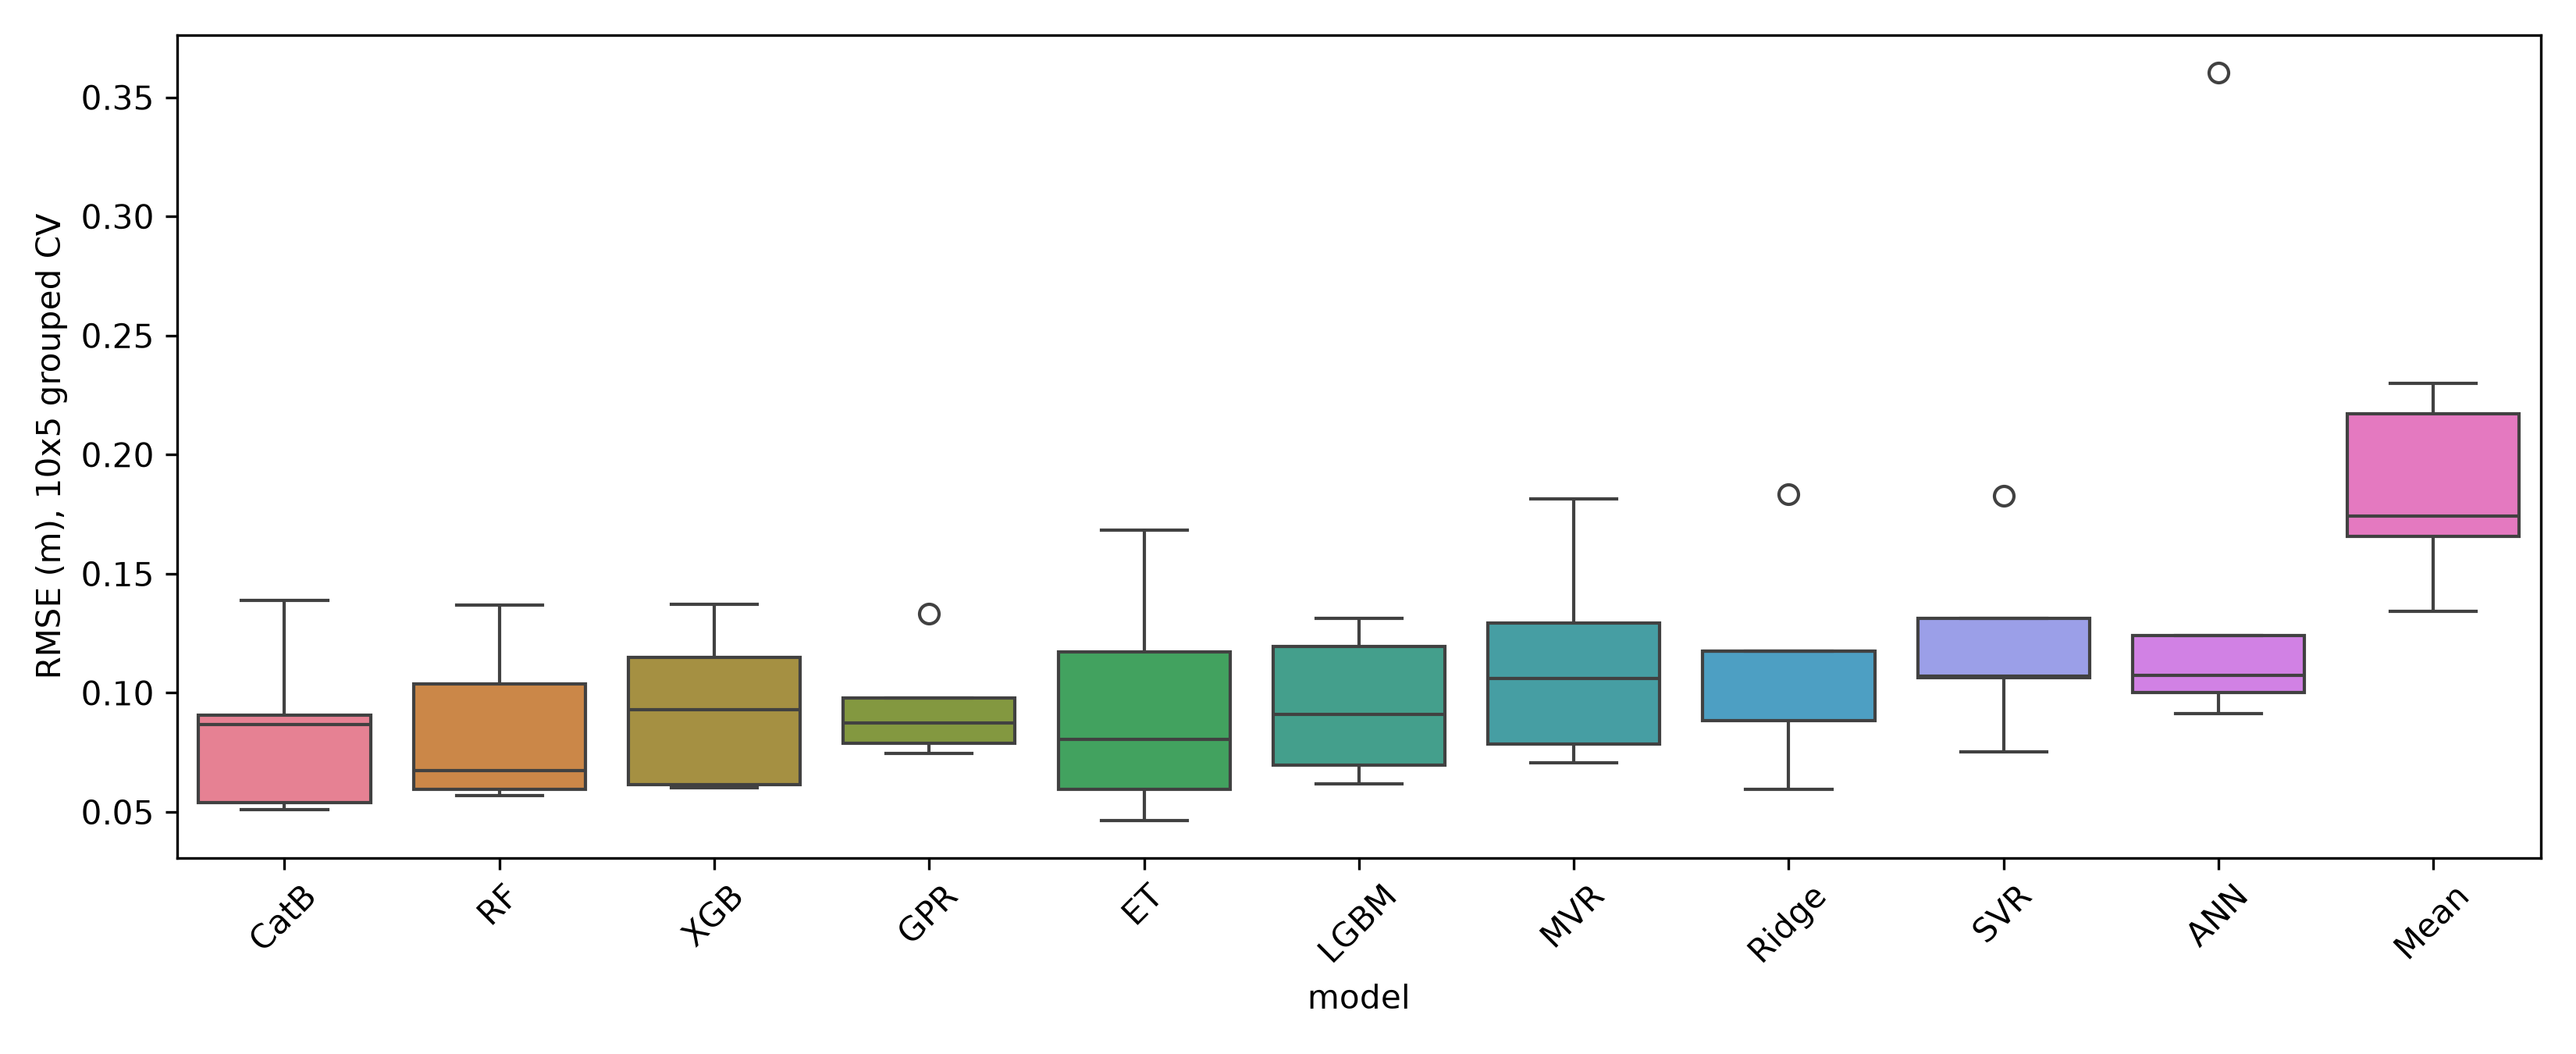
\includegraphics[width=\columnwidth]{figures/F5_cv_boxplot.png}
\caption{Distribution of RMSE across the 50 outer folds of protocol P2 for
each model.}
\label{fig:cvbox}
\end{figure}

\begin{figure*}[t]
\centering
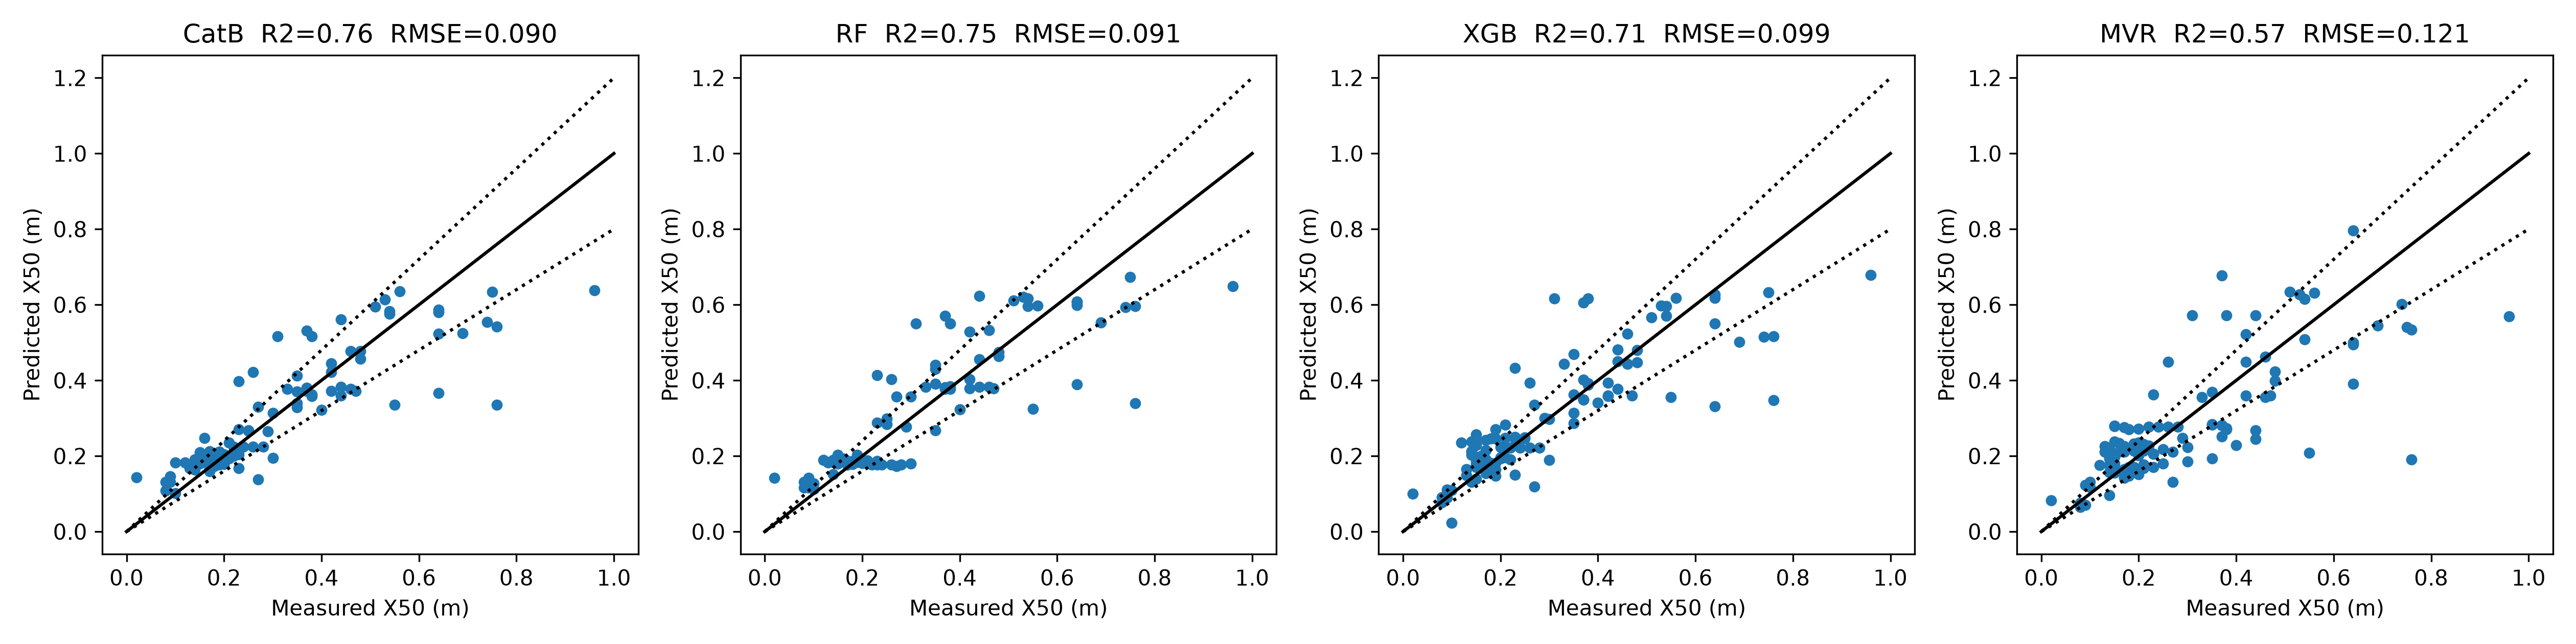
\includegraphics[width=\textwidth]{figures/F6_pred_vs_meas.png}
\caption{Predicted vs.\ measured $X_{50}$ for the top-performing models and
MVR ($\pm20\%$ band shown), pooled out-of-fold predictions, protocol P2.}
\label{fig:predvsmeas}
\end{figure*}

\subsection{Comparison with literature}
Table~\ref{tab:vs_literature} compares our models with the published
Kuznetsov, MVR and ANN predictions of \cite{kulatilake2010} on the 12
shared validation blasts.

\begin{table}[t]
\centering
\caption{Comparison with literature on the 12 shared validation blasts}
\label{tab:vs_literature}
\small
\begin{tabular}{lrrrrrr}
\toprule
 & R2 & RMSE & MAE & MAPE & VAF & a20 \\
Model &  &  &  &  &  &  \\
\midrule
ANN Kulatilake (published) & 0.925 & 0.040 & 0.031 & 10.733 & 93.967 & 0.917 \\
LGBM (ours) & 0.900 & 0.046 & 0.038 & 12.200 & 92.712 & 0.909 \\
CatB (ours) & 0.892 & 0.048 & 0.036 & 10.840 & 92.871 & 0.818 \\
RF (ours) & 0.889 & 0.048 & 0.040 & 12.917 & 90.344 & 0.909 \\
XGB (ours) & 0.889 & 0.049 & 0.038 & 12.850 & 89.442 & 0.909 \\
ET (ours) & 0.854 & 0.056 & 0.036 & 11.565 & 85.657 & 0.818 \\
Ridge (ours) & 0.746 & 0.073 & 0.051 & 13.875 & 84.345 & 0.727 \\
MVR Kulatilake (published) & 0.708 & 0.079 & 0.060 & 18.297 & 81.786 & 0.583 \\
ANN (ours) & 0.668 & 0.084 & 0.053 & 17.063 & 76.562 & 0.727 \\
MVR (ours) & 0.600 & 0.092 & 0.067 & 18.380 & 80.430 & 0.545 \\
GPR (ours) & 0.594 & 0.093 & 0.059 & 18.519 & 59.597 & 0.727 \\
SVR (ours) & 0.280 & 0.124 & 0.077 & 20.278 & 40.739 & 0.455 \\
Kuznetsov (published) & 0.232 & 0.128 & 0.095 & 34.865 & 23.233 & 0.500 \\
Mean (ours) & -0.000 & 0.146 & 0.124 & 43.496 & 0.000 & 0.091 \\
\bottomrule
\end{tabular}

\end{table}

\subsection{Statistical significance}
Table~\ref{tab:significance} reports the corrected resampled $t$-test of
every model against the best-performing model under protocol P2.

\begin{table}[t]
\centering
\caption{Corrected resampled $t$-test vs.\ the best model (protocol P2)}
\label{tab:significance}
\small
\begin{tabular}{lrrr}
\toprule
model & t & p & p\_holm \\
\midrule
ANN & 1.276 & 0.271 & 1.000 \\
ET & 0.877 & 0.430 & 1.000 \\
GPR & 0.617 & 0.571 & 1.000 \\
LGBM & 1.167 & 0.308 & 1.000 \\
MVR & 3.752 & 0.020 & 0.179 \\
Mean & 6.851 & 0.002 & 0.024 \\
RF & 0.083 & 0.938 & 1.000 \\
Ridge & 3.249 & 0.031 & 0.220 \\
SVR & 3.581 & 0.023 & 0.185 \\
XGB & 1.447 & 0.221 & 1.000 \\
\bottomrule
\end{tabular}

\end{table}

% =============================================================================
\section{Interpretability}
% =============================================================================
Figure~\ref{fig:shap} shows the SHAP summary for the best tree-based model.
Table~\ref{tab:importance} reports permutation importance for four
representative models.

\begin{figure}[t]
\centering
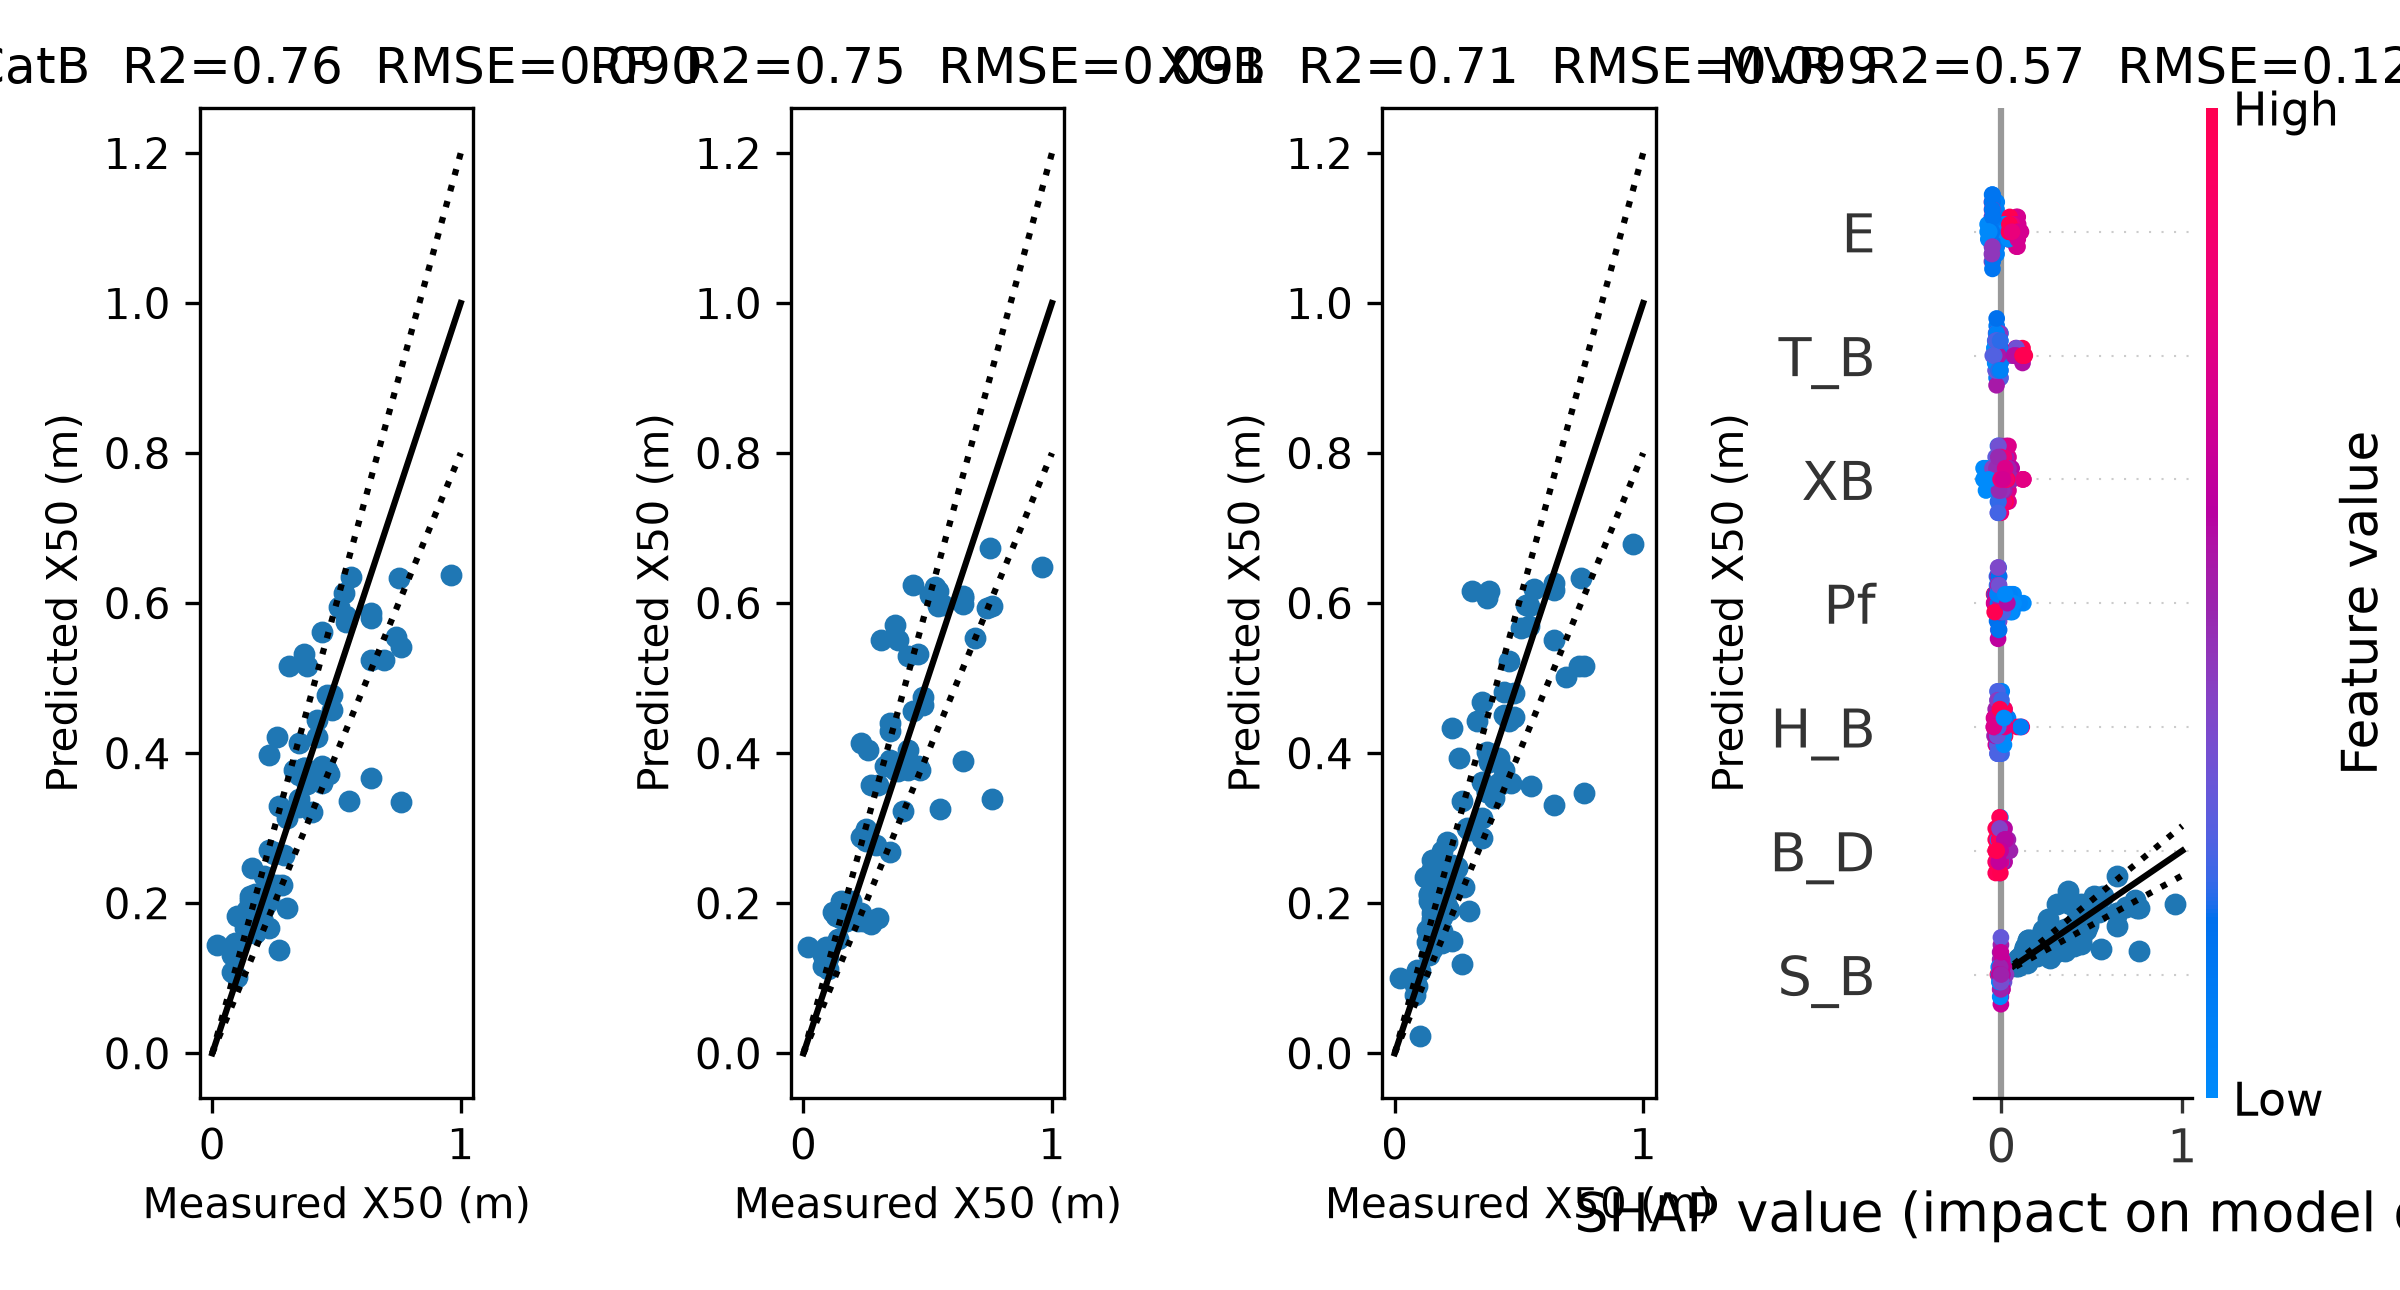
\includegraphics[width=\columnwidth]{figures/F7_shap_beeswarm_XGB.png}
\caption{SHAP beeswarm summary of feature contributions to predicted
$X_{50}$ (XGBoost, fit on all 110 blasts).}
\label{fig:shap}
\end{figure}

\begin{table}[t]
\centering
\caption{Permutation importance (RMSE increase) by model}
\label{tab:importance}
\small
\begin{tabular}{lrrrr}
\toprule
 & XGB & RF & SVR & ANN \\
Feature &  &  &  &  \\
\midrule
S\_B & 0.009 & 0.003 & 0.052 & 0.009 \\
H\_B & 0.038 & 0.015 & 0.079 & 0.095 \\
B\_D & 0.016 & 0.000 & 0.082 & 0.264 \\
T\_B & 0.048 & 0.024 & 0.075 & 0.090 \\
Pf & 0.042 & 0.007 & 0.070 & 0.081 \\
XB & 0.045 & 0.030 & 0.075 & 0.084 \\
E & 0.055 & 0.150 & 0.088 & 0.090 \\
\bottomrule
\end{tabular}

\end{table}

\section{Uncertainty and Practical Tool}
Table~\ref{tab:conformal} reports the empirical coverage and width of 90\%
split-conformal prediction intervals. Figure~\ref{fig:tool} demonstrates a
powder-factor design-tool: for a fixed site and blast geometry, the
predicted $X_{50}$ (with interval) is plotted against powder factor,
allowing a blasting engineer to select $P_f$ for a target fragment size.

\begin{table}[t]
\centering
\caption{90\% split-conformal interval coverage and width}
\label{tab:conformal}
\small
\begin{tabular}{lrrrr}
\toprule
model & P2\_coverage & P2\_interval\_width\_m & P3\_coverage & P3\_interval\_width\_m \\
\midrule
CatB & 0.914 & 0.327 & 0.918 & 0.616 \\
RF & 0.913 & 0.328 & 0.915 & 0.673 \\
ET & 0.913 & 0.375 & 0.914 & 0.541 \\
GPR & 0.911 & 0.379 & 0.912 & 0.764 \\
LGBM & 0.913 & 0.386 & 0.912 & 0.648 \\
XGB & 0.915 & 0.389 & 0.915 & 0.664 \\
MVR & 0.911 & 0.397 & 0.912 & 0.593 \\
Ridge & 0.912 & 0.410 & 0.912 & 0.622 \\
SVR & 0.908 & 0.461 & 0.917 & 0.797 \\
ANN & 0.910 & 0.493 & 0.913 & 1.016 \\
Mean & 0.910 & 0.643 & 0.922 & 0.687 \\
\bottomrule
\end{tabular}

\end{table}

\begin{figure}[t]
\centering
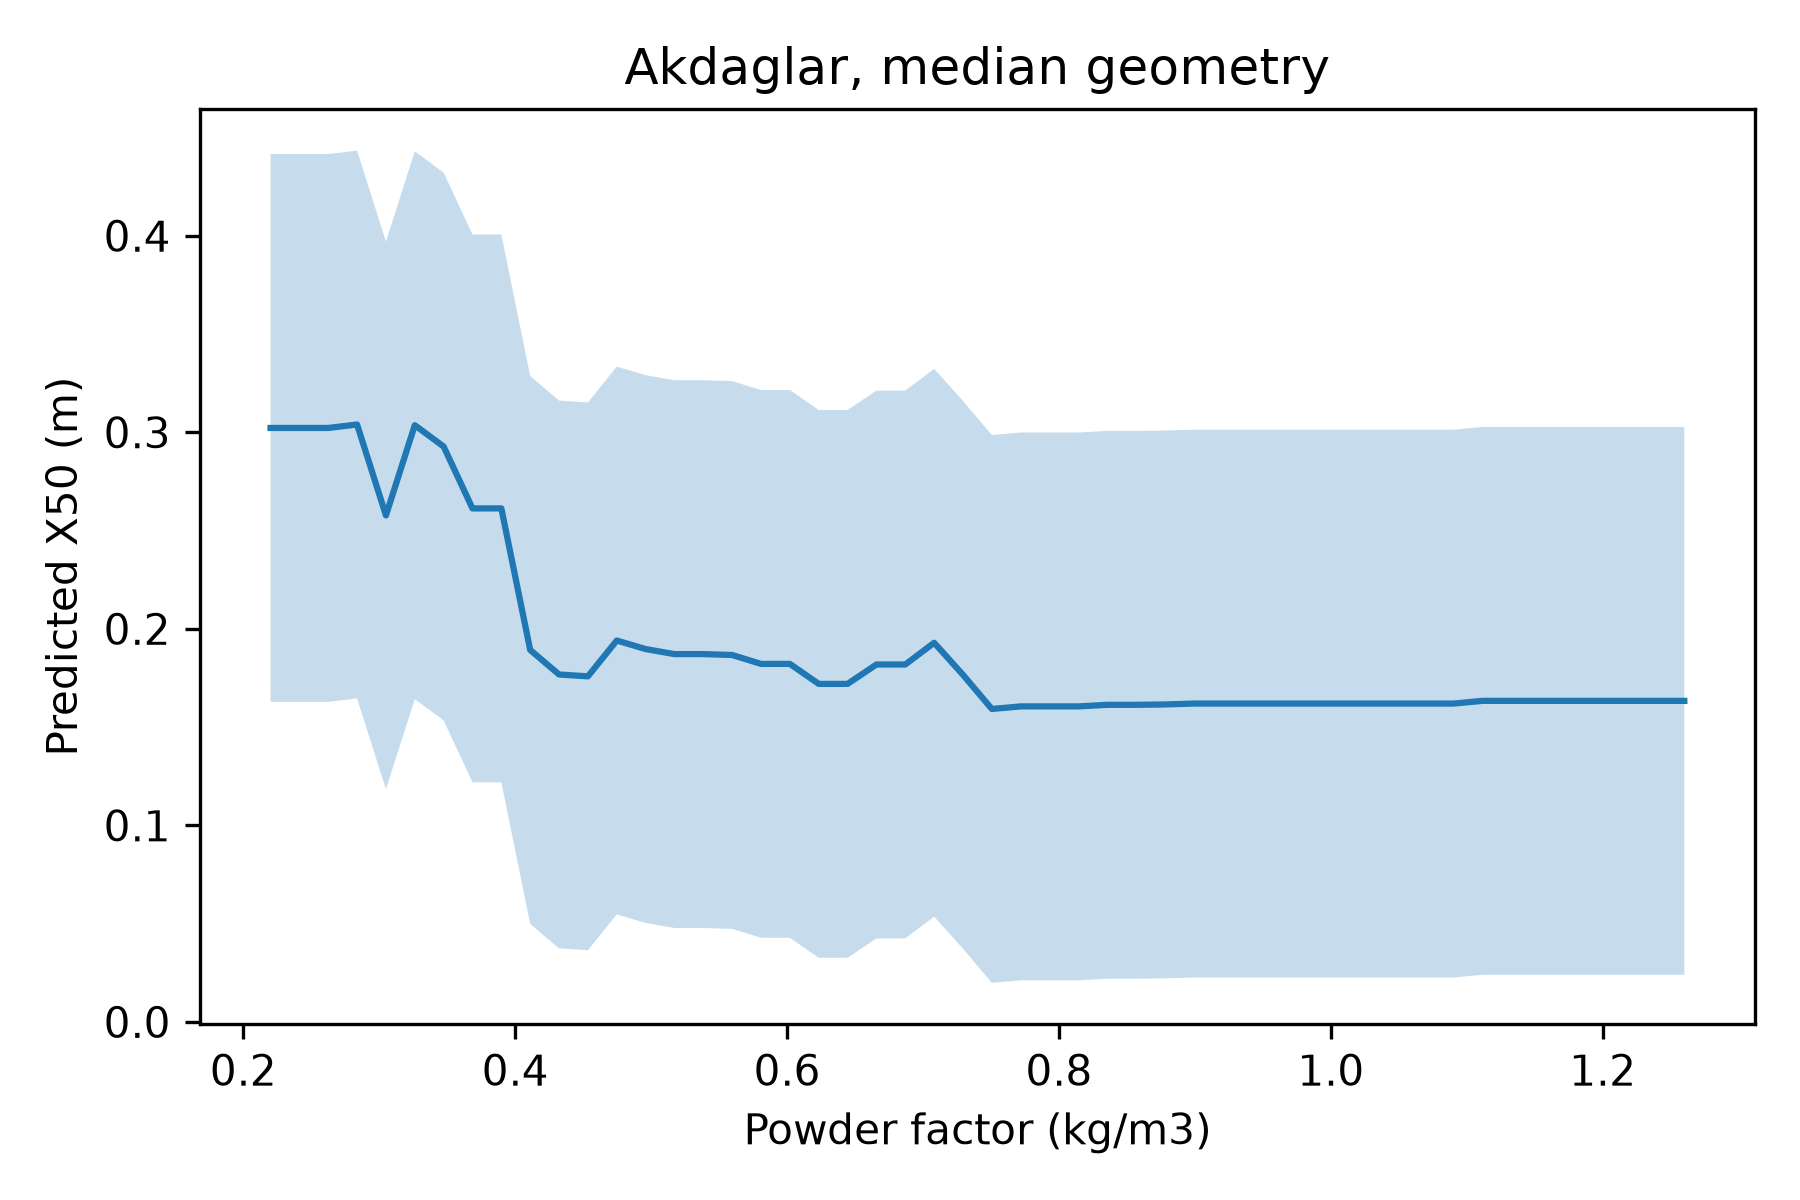
\includegraphics[width=\columnwidth]{figures/F9_design_tool.png}
\caption{Predicted $X_{50}$ vs.\ powder factor for the Akdaglar quarry at
median blast geometry, with 90\% conformal interval.}
\label{fig:tool}
\end{figure}

% =============================================================================
\section{Ablation Studies}
% =============================================================================
Table~\ref{tab:ablations} quantifies the value of the rock-property inputs
($X_B$, $E$) relative to blast-design geometry alone, and the sensitivity
of results to removing the site-proxy feature $E$.

\begin{table}[t]
\centering
\caption{Ablation study: effect of feature subsets on accuracy}
\label{tab:ablations}
\small
\begin{tabular}{llllll}
\toprule
 &  & R2 & RMSE & MAE & MAPE \\
Feature set & Model &  &  &  &  \\
\midrule
\multirow[t]{4}{*}{all_7_features} & MVR & 0.506 $\pm$ 0.241 & 0.113 $\pm$ 0.045 & 0.084 $\pm$ 0.026 & 30.259 $\pm$ 6.753 \\
 & RF & 0.704 $\pm$ 0.197 & 0.083 $\pm$ 0.033 & 0.058 $\pm$ 0.017 & 23.809 $\pm$ 12.116 \\
 & SVR & 0.441 $\pm$ 0.233 & 0.121 $\pm$ 0.04 & 0.083 $\pm$ 0.022 & 30.869 $\pm$ 10.457 \\
 & XGB & 0.65 $\pm$ 0.272 & 0.088 $\pm$ 0.034 & 0.057 $\pm$ 0.017 & 22.695 $\pm$ 12.054 \\
\cline{1-6}
\multirow[t]{4}{*}{geometry_only} & MVR & 0.167 $\pm$ 0.378 & 0.157 $\pm$ 0.055 & 0.121 $\pm$ 0.038 & 55.887 $\pm$ 30.506 \\
 & RF & 0.43 $\pm$ 0.398 & 0.125 $\pm$ 0.041 & 0.093 $\pm$ 0.028 & 52.183 $\pm$ 33.47 \\
 & SVR & 0.332 $\pm$ 0.164 & 0.138 $\pm$ 0.017 & 0.104 $\pm$ 0.017 & 47.226 $\pm$ 27.863 \\
 & XGB & 0.554 $\pm$ 0.292 & 0.111 $\pm$ 0.039 & 0.083 $\pm$ 0.032 & 44.582 $\pm$ 32.919 \\
\cline{1-6}
\bottomrule
\end{tabular}

\end{table}

% =============================================================================
\section{Discussion}
% =============================================================================
\emph{[To be completed once the full-settings Kaggle run is committed.]}
Discuss: (i) which model wins under each protocol and by how much,
referencing the significance test; (ii) the magnitude of the P2$\to$P3
performance drop and what it implies about deployment to a new mine;
(iii) whether SHAP/PDP trends for powder factor, stemming ratio and
in-situ block size agree with blasting-physics expectations
(Section~\ref{sec:methods}), and whether $B/D$ importance is better
explained by site confounding than by blast mechanics; (iv) practical
recommendations for blasting engineers; (v) limitations -- database size
(110 blasts), reliance on ratio-based rather than absolute inputs
(precluding a like-for-like Kuz--Ram comparison outside the 12 shared
blasts), and the third-party transcription of part of the database
(Section~\ref{sec:data}).

% =============================================================================
\section{Conclusions and Future Work}
% =============================================================================
This paper presented a leakage-aware machine-learning benchmark for
bench-blast mean fragment size prediction on a 110-blast, ten-site,
real-world database, comparing eight ML models against the Kuznetsov
equation and multivariate regression under three complementary evaluation
protocols with statistical significance testing. \emph{[Complete with final
headline numbers once the full run is committed.]} Future work includes:
(i) obtaining an independent external test set from a different mine
through direct collaboration with other research groups, since no further
public $X_{50}$ database currently exists; (ii) extending the target from
mean fragment size to the full fragment-size distribution (Rosin--Rammler
/ Swebrec parameters); and (iii) incorporating image-based fragmentation
measurement to enlarge the database at lower cost.

\section*{Data and Code Availability}
The 110-blast database, its provenance log, four Kaggle notebooks
(\texttt{notebooks/01\_eda.ipynb} through \texttt{04\_uncertainty\_ablations.ipynb})
and the LaTeX table-generation script (\texttt{paper/make\_tables.py}) used
to produce every table in this paper are released at
[\emph{repository/Kaggle dataset URL}].

\bibliographystyle{IEEEtran}
\bibliography{references}

\end{document}
